\documentclass[10pt]{article}
\usepackage[spanish]{babel}
\selectlanguage{spanish}
\usepackage[utf8]{inputenc}
\usepackage{graphicx}
\usepackage[lmargin=3cm,rmargin=3cm,tmargin=3cm,bmargin=3cm]{geometry}
\usepackage{amsmath}
\usepackage{amsfonts}
\usepackage{amssymb}
\title{Usando Gnuplot}
\author{Luisa Fernanda Orci Fernandez.}
\date{10 de Marzo del 2015}


\begin{document}

\maketitle
\section{Tiro parabólico en FORTRAN}
El tiro o movimiento kparab[olico  es aquel realizado por algún objeto y describe una trayectoria en forma de parábola.
En esta actividad se hizo un programa en FORTRAN para calcular la posición en ciertos instantes de tiempo de un objeto que fue lanzado con tiro parabóilico. El programa calcula la "x" y "y" máxima, así como el tiempo total de vuelo. Para calcular esto, se le pide al usuario un ángulo inicial, así como la velocidad inicial. \\
Para realizar estos calculos utilizamos las formulas:
$$x = v_0tcos(\theta)$$
$$y = v_otsin(\theta)- \frac{1}{2}gt^2$$

\subsection{Código utilizado}
El código utilizado para calcular el tiro parabólico fue:

\begin{verbatim}
!************************************************ 
!This program plots projectile motion of an object.
!The program requires user input for initial velocity
!and angle of the object.The algorithm uses a time
!step of 0.01 second i.e. it calculates object's 
!location in the x and y plane every 0.01 second.
!**********By: Waleed Ishaque, 2013**************  
program tiro_parabolico
   implicit none
   !Defining constants: 
   real, parameter :: pi = 3.14159265359
   real :: velocidad, angulo, tiempo, radianes, vx, vy, xm, ym
   real :: tiempoesperado, incrementoTiempo
   real, parameter :: gravedad = 9.81
   real:: x(100),y(100)

   integer :: i, ret

   ! donde g es la aceleracion de la gravedad, pi is "pi"
   ! v es la velocidad inicial del objeto
   ! a es el angulo de tiro, r es el mismo angulo, pero en radianes
   ! t es el tiempo
   ! 'x' y 'y' son cordenadas del objeto durante el tiro
   !Seek user input

   write(*,*) 'Dame el ángulo inicial de tiro del proyectil en grados (Real)'
   read *, angulo

   write(*,*) 'Dame la velocidad inicial del proyectil en m/s (Real) '
   read *, velocidad


   radianes = (angulo*pi)/180.0

   ! Calculando las velocidades en los 2 ejes
   vx=(velocidad)*(cos(radianes))
   if (vx < 0) then
      vx = -1*vx
   end if
   vy=(velocidad)*(sin(radianes))

   print *, 'La velocidad inicial en x es de ',  vx
   print *, 'La velocodad inicial en y es de ', vy
    
   !open .dat file and start writing on it using the algorithm
   open(1, file='tiro.dat')

   x=0
   y=0


   ! Cuanto tiempo me voy a tardar?
   tiempoesperado = 2*velocidad*sin(radianes)/gravedad
   incrementoTiempo = tiempoesperado/100


   tiempo = 0.0
   do i=1,100
      !displacement of object in x and y direction
      !tiempo = (float(i)*0.01)
      tiempo = tiempo + incrementoTiempo
      x(i) = vx*tiempo
      y(i) = (vy*tiempo) - (0.5*gravedad*tiempo*tiempo)

      !write output in file "proj.dat" for plotting
      write(1,*) x(i), y(i)
        
      !kill the loop when the object hits the ground
      if (y(i)<0) exit
   end do
   close(1)

   !close file
   ym = (vy**2)/(19.6)
   xm = x(i-1)
   if (vx<0) then
      xm = 0
   end if
   !resultados en pantalla
   write(*,*) '^^^^^^^^^^^^^^^^^^^^^^^^^^^^^^^^^^^^^^^^^^^^^^^^^^^^^^^^^^^^^^^'
   write(*,*) 'Un proyectil con una velocidad inicial de ', velocidad, 'm/s'
   write(*,*) 'y con un ángulo de tiro de ', angulo, 'grados'
   write(*,*)  'Alcanzará una h máxima de ', ym, 'metros'
   write(*,*) 'Su alcanze horizontal sera de', xm, 'metros'
   write(*,*) 'y durará en el aire un tiempo de', tiempo, 'segundos'
   write(*,*) '== Tiempo esperado de vuelo : ', tiempoesperado, 's'

   ret = SYSTEM('gnuplot graph.txt')

end program tiro_parabolico
\end{verbatim}
\newpage

\subsection{Terminal y gráficas}
A continuación, una muestra del programa probado para 90, 60, 30 y 0 grados.
\subsubsection{90 grados}
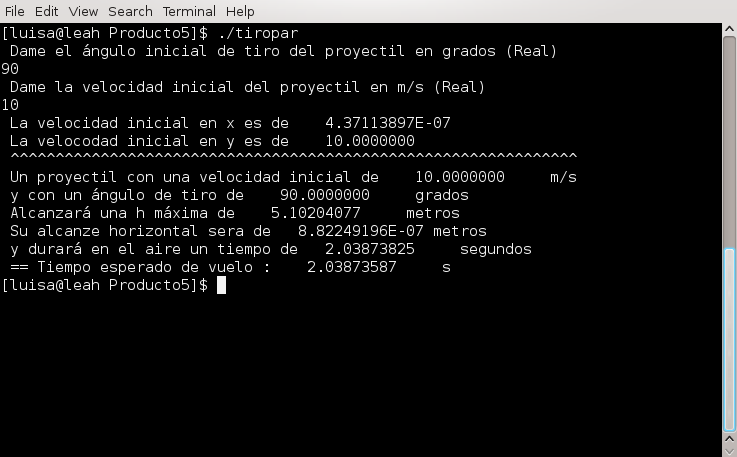
\includegraphics[scale=0.6]{screen90.png} \\
\\
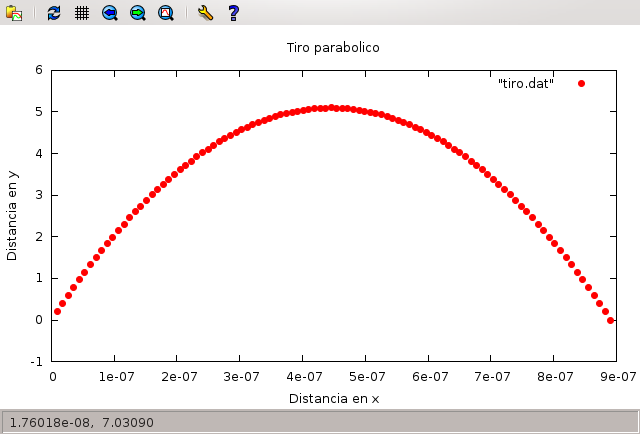
\includegraphics[scale=0.6]{grafica90.png}

\newpage

\subsubsection{60 grados}
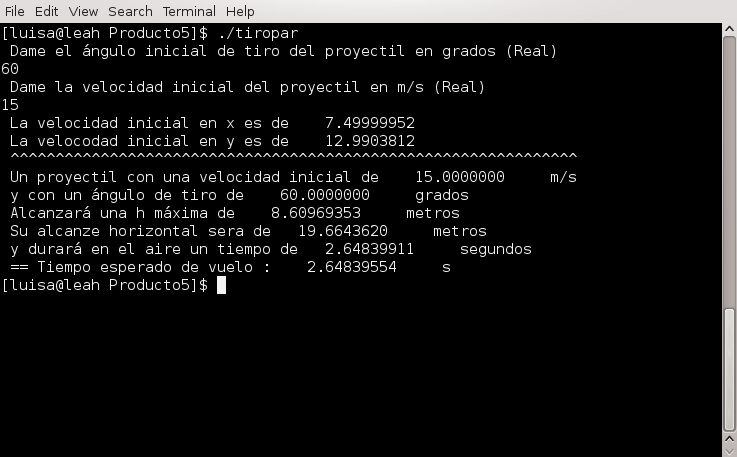
\includegraphics[scale=0.6]{screen60.png} \\
\\
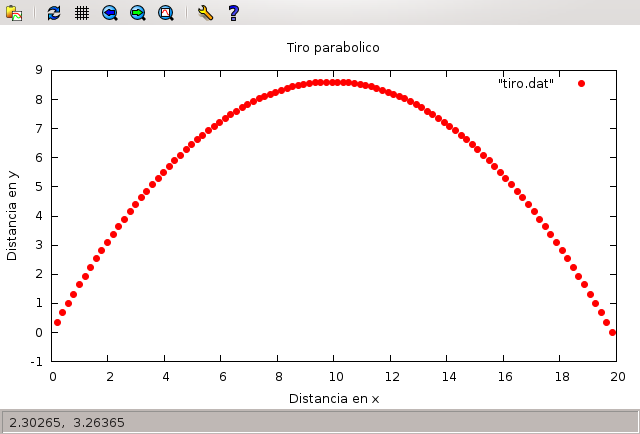
\includegraphics[scale=0.6]{grafica60.png} 

\newpage

\subsubsection{30 grados}
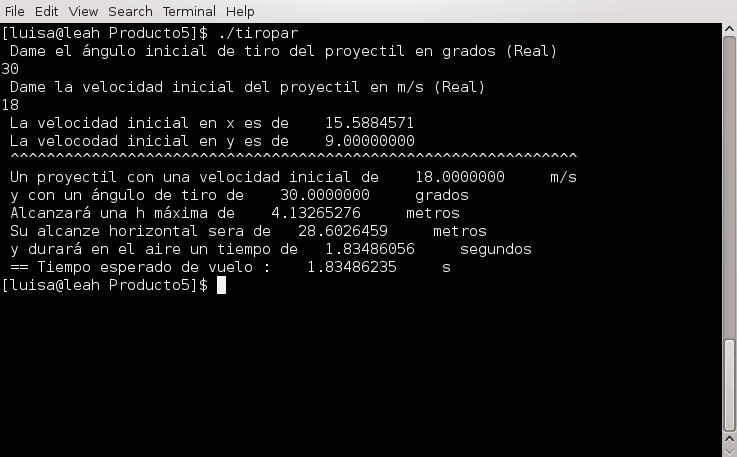
\includegraphics[scale=0.6]{screen30.png} \\
\\
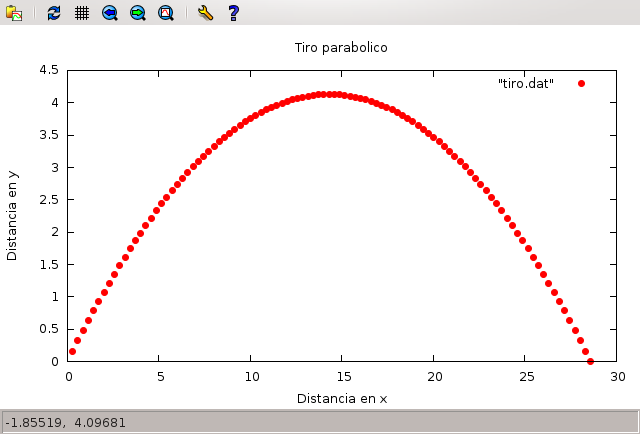
\includegraphics[scale=0.6]{grafica30.png}

\newpage

\subsubsection{0 grados}
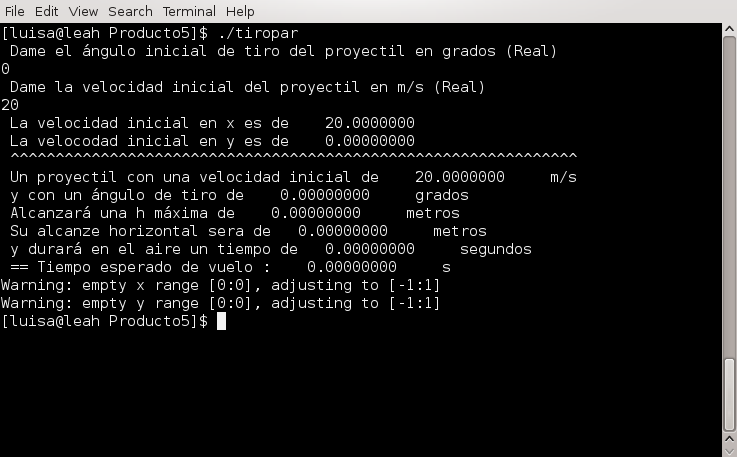
\includegraphics[scale=0.6]{screen0.png} \\
\\
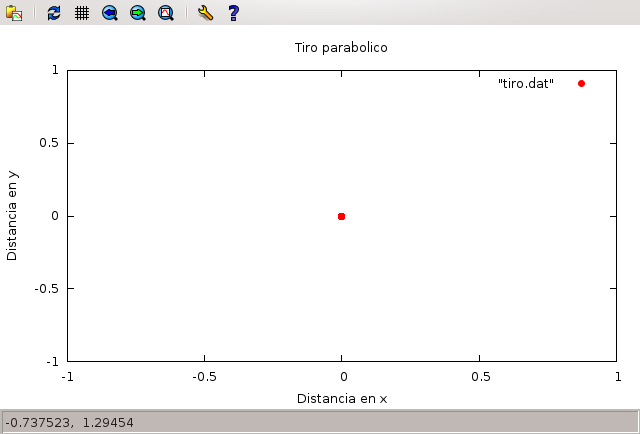
\includegraphics[scale=0.6]{grafica0.png}


\end{document}